\documentclass[preprint,12pt]{elsarticle}
\usepackage[a4paper,left=2.5cm,right=2.5cm,top=2.5cm,bottom=3cm,footskip=1.6cm]{geometry}
\usepackage{array}
\usepackage[hidelinks]{hyperref}
\usepackage{xr-hyper}
\externaldocument{../main}
\biboptions{numbers,sort&compress}
\journal{Reliability Engineering \& System Safety}
\emergencystretch=3em
\renewcommand{\topfraction}{0.85}
\usepackage{amsmath,amssymb,amsthm,booktabs,graphicx,xcolor,adjustbox}
\usepackage{tikz}
\usetikzlibrary{arrows.meta,decorations.pathreplacing,calc,fit,backgrounds,shadows}
\newtheorem{theorem}{Theorem}
\newtheorem{proposition}{Proposition}
\newtheorem{lemma}{Lemma}
\newtheorem{corollary}{Corollary}
\newtheorem{definition}{Definition}
\newtheorem{remark}{Remark}
\theoremstyle{definition}
\newcommand{\todo}[1]{\textcolor{red}{[TODO: #1]}}
\newcommand{\E}{\mathbb{E}}
\newcommand{\Binfo}{\mathcal{B}_{\mathrm{info}}}
\newcommand{\Istate}{\mathcal{I}_{\mathrm{state}}}
\newcommand{\Ikin}{\mathcal{I}_{\mathrm{kin}}}
\newcommand{\etaPIE}{\eta_{\mathrm{info}}}
\DeclareMathOperator{\Mon}{Mon}
\DeclareMathOperator{\Var}{Var}

\begin{document}
\begin{center}\textbf{Benchmark details for ``Information Budgets of Trajectory Health Indicators for Remaining Useful Life Prediction''}\end{center}
\noindent This document collects the benchmark material that supports Section~\ref{sec:empirical} of the paper and was moved out of its appendices: the learned encoders and the predictive distribution, the data, protocols and evidence tiers, the detailed benchmark tables, and the initial benchmark protocol P1. Sections, tables and references of the paper are cited by their numbers in the paper; the bibliography is that of the paper.

\renewcommand{\thesection}{S\arabic{section}}
\renewcommand{\thetable}{S\arabic{table}}
\renewcommand{\thefigure}{S\arabic{figure}}
\section{Estimators used in the benchmark}
\label{sec:pgib}
This appendix describes the estimators compared in Section~\ref{sec:empirical}. The path-space objective follows from the theory; the architectures and the calibration are design choices.

\subsection{Path-space objective}
We seek a causal stochastic encoder, the \emph{physics-guided information bottleneck} (PGIB), $q_\theta(H_{1:t}\mid\mathbf{X}_{1:t})=\prod_{k=1}^{t}q_\theta(H_k\mid H_{k-1},\mathbf{X}_{1:k})$, whose increments are Gaussian, $\mathcal N\big(H_{k-1}+u_\theta(\mathbf{X}_{1:k})\Delta t,\;s_\theta^2(\mathbf{X}_{1:k})\Delta t\big)$, with a positive velocity $u_\theta$ (enforced by a softplus output) and a variance $s_\theta^2$. The encoder is regularised towards a physics prior $p_\phi(H_{1:t})=\prod_k\mathcal N\big(H_{k-1}+\nu(H_{k-1};\phi)\Delta t,\;\sigma_B^2\Delta t\big)$, $H_0\equiv0$, where $\Delta t$ is the time step, $\nu$ a state-dependent drift with parameters $\phi$, and $\sigma_B$ the diffusion coefficient.

\begin{proposition}[Compression bound and path-space KL]
\label{prop:kl}
For any prior $p_\phi$, $I(\mathbf{X}_{1:t};H_{1:t})\le \E_{\mathbf{X}}\big[D_{\rm KL}(q_\theta(H_{1:t}\mid\mathbf{X}_{1:t})\,\|\,p_\phi(H_{1:t}))\big]$, and for the Gaussian factorisation above the divergence is exactly
\begin{equation}
D_{\rm KL}=\frac12\sum_{k=1}^{t}\E_{q_\theta(H_{k-1}\mid\mathbf{X}_{1:k-1})}\!\left[\frac{s_\theta^2}{\sigma_B^2}-1-\ln\frac{s_\theta^2}{\sigma_B^2}+\frac{(u_\theta-\nu(H_{k-1};\phi))^2\,\Delta t}{\sigma_B^2}\right].
\end{equation}
\end{proposition}
\begin{proof}
The first claim is the standard variational upper bound of the information bottleneck \cite{tishby2000,alemi2017,poole2019}: $I(\mathbf{X};H)=\E_{\mathbf{X}}D_{\rm KL}(q(H\mid\mathbf{X})\|q(H))\le\E_{\mathbf{X}}D_{\rm KL}(q(H\mid\mathbf{X})\|p(H))$ because the difference is $D_{\rm KL}(q(H)\|p(H))\ge0$. The chain rule of the KL divergence \cite[Sect.~2.5]{cover2006} over the causal factorisation gives $\sum_k\E_{q(H_{k-1}\mid\cdot)}D_{\rm KL}(q(H_k\mid H_{k-1},\mathbf{X}_{1:k})\|p_\phi(H_k\mid H_{k-1}))$, and the Gaussian KL with means differing by $(u_\theta-\nu)\Delta t$ and variances $s_\theta^2\Delta t$, $\sigma_B^2\Delta t$ yields the summand (the Gaussian KL of the variational autoencoder \cite{kingma2014}).
\end{proof}
The training objective is $\mathcal{L}_{\rm PGIB}=\mathcal{L}_{\rm FHT}+\beta\,D_{\rm KL}$, where $\beta$ weights the compression term and $\mathcal{L}_{\rm FHT}$ is the negative log-likelihood of the observed failure time under the predictive distribution below, a variational surrogate for $-I(T_t;H_{1:t})$ in the sense of \cite{alemi2017} (Algorithm~1 in Appendix~\ref{app:data}).

\subsection{Predictive distribution}
Let the posterior of the unit's drift $\mu$ given the HI increments be $\mathcal N(\hat\mu_t,\sigma_{\mu,t}^2)$ (conjugate update). Marginalising the inverse-Gaussian distribution over $\mu$ (a Gaussian integral; random-drift Wiener models are treated in \cite{gebraeel2005,wang2010}) gives
\begin{equation}
p(T_t=\tau\mid H_{1:t})=\frac{a}{\sqrt{2\pi\tau^3(\sigma_B^2+\sigma_{\mu,t}^2\tau)}}\exp\!\left(-\frac{(a-\hat\mu_t\tau)^2}{2\tau(\sigma_B^2+\sigma_{\mu,t}^2\tau)}\right),\qquad a=D_{\rm fail}-\hat D_t .
\label{eq:mixig}
\end{equation}
Here $\sigma_B^2$ is the aleatoric and $\sigma_{\mu,t}^2\tau$ the epistemic contribution to the effective diffusion; as $t$ grows $\sigma_{\mu,t}^2\to0$ and (\ref{eq:mixig}) reduces to the inverse-Gaussian distribution. It is a defective density, the missing mass being the probability that the threshold is never reached, which can happen only for a non-positive drift, and $\hat D_t$ is the filtered state rather than the raw HI value, which avoids the degeneracies of non-monotone paths. The distribution was checked against numerical integration of the mixture (Section~\ref{sec:physnum}).

\subsection{Observation-corrected and regime-aware encoders}
\label{sec:kf}
The encoder above integrates a positive velocity, $H_k=H_{k-1}+u_\theta\Delta t+\dots$, so nothing anchors the level to the observations (Section~\ref{sec:accum}). The observation-corrected encoder, PGIB-KF (KF: Kalman filter), therefore adds a direct level estimate $l_k=f_l(\mathbf h_k)$ and a learned gain $\omega_k=\mathrm{sig}(f_\omega(\mathbf h_k))\in(0,1)$ to the encoder features $\mathbf h_k$ (here $\mathrm{sig}$ is the logistic function and $\epsilon_k\sim\mathcal N(0,1)$ the encoder noise),
\begin{equation}
H_k=(1-\omega_k)\big(H_{k-1}+u_k+s_k\epsilon_k\big)+\omega_k\,l_k .
\end{equation}
Given $H_{k-1}$ this is again a Gaussian transition with drift $u^{\rm eff}_k=(1-\omega_k)u_k+\omega_k(l_k-H_{k-1})$ and standard deviation $s^{\rm eff}_k=(1-\omega_k)s_k$, so Proposition~\ref{prop:kl} applies unchanged: the bottleneck now prices the use of the observation beyond what the physics prior allows ($\beta\to\infty$ gives $\omega\to0$, a pure integrator). The HI is no longer monotone by construction.

The error accumulation of an integrating encoder and its correction by the gain $\omega$ are analysed in Proposition~\ref{prop:accum}.

By Proposition~\ref{prop:regime}, a regime-blind estimator has an error floor, and per-regime normalisation removes the offsets but not the gains. The regime-aware variant, \emph{PGIB-KFR}, therefore places the regime in the \emph{observation} model, where the proposition locates it. The process model is shared, whereas the level estimate $l_k$ and the gain $\omega_k$ use regime-specific linear heads on the encoder features, $l_k=\mathbf h_k^\top\mathbf W^{l}_{r_k}+b^{l}_{r_k}$ and $\omega_k=\mathrm{sig}(\mathbf h_k^\top\mathbf W^{\omega}_{r_k}+b^{\omega}_{r_k})$, where $r_k$ is the regime, which is also an input of the encoder. The regimes are the clusters of the standardised operating settings. With a single regime PGIB-KFR reduces to PGIB-KF, which we check on the single-regime subsets.

\subsection{Calibrated predictive distribution with age fusion}
\label{sec:fusion}
Because the age is always known (Theorem~\ref{thm:bound}(c)), the HI-based distribution $p_{\rm HI}(\tau)$, which is (\ref{eq:mixig}) with diffusion $c\,v_t$ and drift variance $c\,v_t/w_t$, is pooled log-linearly \cite{genest1986,hinton2002} with an age-based lifetime distribution. Here $v_t$ is the variance of the HI increments over the trailing window of length $w_t$ for non-learned HIs and the learned $\sigma_B^2$ for the bottleneck models, and $c>0$ is a calibration multiplier. The age-based distribution is $p_{\rm age}(\tau\mid t)=f_L(t+\tau)/S_L(t)$, the log-normal lifetime density $f_L$ with survival function $S_L$ \cite{meeker1998}, fitted on training lifetimes (log-scale floor $0.15$) conditioned on survival to age $t$. The pooled distribution is
\begin{equation}
p(\tau)\;\propto\;p_{\rm HI}(\tau)^{w_{\rm h}}\;p_{\rm age}(\tau\mid t)^{w_{\rm a}},\qquad (c,w_{\rm h},w_{\rm a})\in\mathcal G,
\end{equation}
on a finite grid $\mathcal G$ ($c\in[10^{-2},10^{2}]$ on a log scale, ten pairs $(w_{\rm h},w_{\rm a})$ including $(1,0)$ and $(0,1)$). The parameters minimise the negative log-likelihood of the true RUL, a strictly proper scoring rule \cite{gneiting2007}, on HI paths produced \emph{out of sample}: each HI construction is fitted on all but one training unit and applied to the left-out unit; the test unit is never used. The family contains the plain HI-based distribution and the age-only distribution, so in-sample the pooled distribution cannot do worse than either. Weights below one temper the corresponding distribution and widen the predictive interval, which the otherwise under-covering plain distribution requires. The pooling is a calibration procedure, not a Bayes-exact fusion, which would also require conditional independence of the HI and the age given the RUL, and division by the marginal distribution of the RUL. The same predictor is used for every HI, and a variant without fusion ($w_{\rm a}=0$) is reported for each HI, so that the effects of the HI and of the fusion can be separated.

\section{Data, protocols and evidence tiers}
\label{app:data}
\paragraph{Data} Public run-to-failure collections were used: NASA PCoE cells B0005, B0006, B0007 and B0018 \cite{saha2007}; CALCE CS2 cells \cite{he2011}; the FEMTO-ST/PRONOSTIA bearings \cite{nectoux2012}; the NASA IMS bearings \cite{lee2007,qiu2006}; and the C-MAPSS turbofan engines \cite{saxena2008}. For batteries, the capacity is used only to define the EOL and is never an input. The EOL is the first cycle at which the rolling-median capacity falls to $75\%$ (NASA) or $80\%$ (CALCE) of the initial capacity; an absolute threshold of $1.4$~Ah was not used because cell B0007 never reaches it. The lifetimes are $127$, $73$, $162$ and $100$ cycles (NASA) and $542$, $499$, $572$ and $600$ cycles (CS2\_35 to CS2\_38); the data are truncated at the EOL, and CALCE features are averaged over blocks of $4$ cycles. Six per-cycle features are extracted from the charge and discharge records: constant-current time, constant-voltage time, height and voltage of the incremental-capacity peak, mean discharge temperature (NASA) or voltage drop at discharge onset (CALCE), and the discharge voltage at a fixed time ($600$~s for NASA, $1200$~s for CALCE).

Further cells were screened by inclusion rules fixed before running any model (scripts and outputs are supplied). A NASA cell had to be at $24^\circ$C, have at least $100$ discharge cycles, be discharged at a roughly constant $1.4$ to $2.1$~A, start between $1.5$ and $2.1$~Ah and reach the $75\%$ EOL; only the four cells above qualify. Among the CALCE cells, CS2\_5, 24 and 25 are partial-discharge tests, CS2\_9 is discharged at a rate of $2$C (twice the nominal capacity per hour), and CS2\_3, 6 and 7 are short or follow other protocols, so none was used. CS2\_33 and CS2\_34 have the same chemistry and run to the EOL ($485$ and $479$ cycles) but are discharged at $0.55$~A; they are used only in a separate six-cell experiment, labelled protocol-heterogeneous, and the four-cell set remains the primary one.

For bearings, each run ends at failure, so EOL is the last snapshot. Condition 1 (nominally $1800$~rpm, $4000$~N; Bearing1\_1--1\_7) and condition 2 ($1650$~rpm, $4200$~N; Bearing2\_1--2\_7) are evaluated separately, each with $7$ units from the learning and the full test sets; condition 3 has only $3$ units and was not used. The lifetimes are $2803$, $871$, $2375$, $1428$, $2463$, $2448$, $2259$ snapshots (condition 1) and $911$, $797$, $1955$, $751$, $2311$, $701$, $230$ snapshots (condition 2), each snapshot covering $0.1$~s of $25.6$~kHz acceleration every $10$~s. Eight features are computed per snapshot: logarithm of the root mean square (RMS), kurtosis, crest factor and spectral entropy of the horizontal and of the vertical channel. Features are averaged over blocks of $20$ (condition 1) or $8$ (condition 2) snapshots, and the RUL is reported in snapshots.

Evaluation is leave-one-unit-out: each unit in turn is held out, the remaining units are used for training (three for NASA and four-cell CALCE, five for six-cell CALCE, six for each bearing condition), and metrics are computed at every step in the window $40$--$90\%$ of life and pooled over the held-out units.


\paragraph{Further collections} FEMTO condition 3 ($1500$~rpm, $5000$~N; Bearing3\_1--3\_3, with $515$, $1637$ and $434$ snapshots, block length $10$) and the NASA IMS bearings were reserved and used only as confirmation sets. For IMS the four bearings that failed (Test~1 bearings 3 and 4, Test~2 bearing 1, Test~3 bearing 3; $2156$, $2156$, $984$ and $6324$ snapshots of $1$~s at $20$~kHz every $10$~min) are used with one accelerometer channel each and four features per snapshot (log RMS, kurtosis, crest factor, spectral entropy), averaged over blocks of $20$ snapshots. For C-MAPSS we use the single-condition subsets FD001 and FD003 ($100$ training engines run to failure and $100$ truncated test engines with the official RUL labels each); the $14$ informative sensors are standardised with training statistics. The $100$ training engines are split by identifier into $80$ engines to fit the HI constructions and $20$ (identifier divisible by five) to select the bottleneck configuration and to calibrate the predictor; the test engines are predicted once at their last observed cycle, and $95\%$ bootstrap intervals are computed over engines. The multi-regime subsets FD002 ($260$ training and $259$ test engines) and FD004 ($249$ and $248$) have six operating regimes; for them the only change is that sensors are standardised within regime, the six regimes being the clusters of the standardised operating settings found on the fitting engines (the clusters recover the six discrete settings exactly), the same preprocessing being applied to every method; the split is by identifier as above, with $208$ and $200$ fitting engines.

\paragraph{Methods} To isolate the effect of HI construction, every HI is mapped to the same scale and passed to the same calibrated predictor of Appendix~\ref{sec:fusion}. The sensor features are standardised, and each HI is mapped by an affine map $H\mapsto(H-H_{\rm s})/(H_{\rm e}-H_{\rm s})$, where $H_{\rm s}$ and $H_{\rm e}$ are the averages, over the \emph{training} units only, of the mean of the first five and of the last five HI values of a unit (the end of life of a training unit is known); the standardisation, the PCA direction, the combination weights of the Geo-opt HI, the encoders and the affine map are all fitted on the training units and applied unchanged to the test unit, whose own end-of-life value is never used. The PGIB scale is set by its end-of-life penalty on the training units. The predictor of Appendix~\ref{sec:fusion} then uses: the mixed inverse-Gaussian distribution (\ref{eq:mixig}) with the drift taken from the slope of the smoothed HI over a trailing window of $\max(10,0.25t)$ steps, pooled with the age-based distribution. The parameters $(c,w_{\rm h},w_{\rm a})$ are chosen on HI paths that are out of sample for the HI construction (leave-one-training-unit-out for the small sets, the $20$ calibration engines for C-MAPSS). Implementation details of the compared HIs: the Geo-opt HI is found by differential evolution; the $\beta$-VAE uses a causal gated recurrent unit (GRU) encoder with a one-dimensional latent variable and a Gaussian prior; VIB is the PGIB with a zero-drift prior, that is, without physics; the PGIB has the state-dependent drift $\nu(H;\phi)=\phi_1\exp(\phi_2H)$ (Appendix~\ref{sec:kf} for PGIB-KF). For the bottleneck models, the compression weight $\beta\in\{0.03,0.3,3,30\}$ and the encoder (GRU or causal feed-forward window network) are selected by inner leave-one-training-unit-out validation of the predictive negative log-likelihood, with at most three inner folds when more than five training units are available; for PGIB-KF only $\beta\in\{0.03,0.3,3\}$ is searched. The held-out unit is never used. Learned models use three seeds, and the other HIs are deterministic. The sensor-free reference is the age-based distribution $p_{\rm age}$ of Appendix~\ref{sec:fusion}. The metrics are the RMSE and the mean absolute error (MAE) of the median prediction, the prediction interval coverage probability (PICP) and normalised average width (PINAW) of the $95\%$ interval, and the continuous ranked probability score (CRPS) \cite{gneiting2007}. For C-MAPSS the asymmetric score is $\sum_i(e^{-d_i/13}-1)$ for $d_i<0$ and $\sum_i(e^{d_i/10}-1)$ for $d_i\ge0$, summed over engines, with $d_i$ the predicted minus the true RUL \cite{saxena2008}.

\paragraph{Protocol history and evidence tiers} The study proceeded in five protocols, which determine how the numbers can be read. P1 (Appendix~\ref{app:initial}) showed that the integrating encoder under-covers and that the age-only baseline is competitive. P2 added out-of-sample calibration, age fusion and a prediction grid independent of the test unit; it was frozen, with the file hash recorded, before it was run on the confirmation sets (FEMTO condition 3 and IMS). On C-MAPSS FD001, P2 showed that the integrating encoder is considerably worse than simple HIs even with $80$ training engines. The diagnosis of Proposition~\ref{prop:accum} led to P3, the observation-corrected PGIB-KF, which was frozen and run once on FD003, a subset not used before, and then, with regime-wise preprocessing, once on FD002 and FD004. (A first launch used only the first $100$ training engines because the identifier list was fixed in the script; it was stopped before any result was produced, and the script and the recorded hash were corrected.) P4 added the regime-aware encoder and a regime-specific ridge baseline and was run once on each subset, the choice between PGIB-KF and PGIB-KFR and of $\beta$ being made on the calibration engines only; FD002 and FD004 are therefore development sets for P4, and no independent multi-regime data set was available (the successor N-CMAPSS has only six to ten units per subset). Because the differences between learned encoders and simple HIs were of the size of the seed-to-seed variability, P5 retrained the learned encoders on the four subsets with ten fresh seeds, keeping architecture, $\beta$ and calibration fixed; it supersedes the three-seed results where they disagree. The evidence tiers are: (i) \emph{independent confirmation}: C-MAPSS FD003, FD002 and FD004 for P3 (not for P4), and FEMTO condition 3 and IMS for P2 (not for P3); (ii) \emph{development}: NASA, CALCE (four and six cells), FEMTO conditions 1 and 2 and C-MAPSS FD001, which informed the design and whose results are therefore not unbiased estimates of out-of-sample performance.

\begin{table}
\caption{Algorithm 1: training of the PGIB and Bayesian FHT prognostics (Appendix~\ref{sec:pgib}).}
\centering
\begin{tabular}{p{0.95\textwidth}}
\hline
\textbf{Input:} training sequences $\{\mathbf{X}^{(n)}_{1:T_n},T^{(n)}\}$, threshold $D_{\rm fail}=1$, compression weight $\beta$, step $\Delta t$. \textbf{Output:} $q_{\theta^*}$, $(\phi^*,\sigma_B^*)$, predictive distribution (\ref{eq:mixig}).\\
\hline
1. Causal encoder (temporal convolutional network or GRU): $u_\theta,s_\theta\leftarrow\mathrm{softplus}(\cdot)$ from $\mathbf{X}_{1:k}$.\\
2. Sample the path by reparametrisation: $H_k=H_{k-1}+u_\theta\Delta t+s_\theta\sqrt{\Delta t}\,\epsilon_k$, $\epsilon_k\sim\mathcal N(0,1)$, $H_0=0$.\\
3. Conjugate drift update from $\Delta H_{1:t}$ to obtain $(\hat\mu_t,\sigma^2_{\mu,t})$.\\
4. $\mathcal{L}_{\rm FHT}=-\ln p(T_t\mid H_{1:t})$ from (\ref{eq:mixig}); $\mathcal{L}_{\rm KL}$ from Proposition~\ref{prop:kl}.\\
5. Update $(\theta,\phi,\sigma_B)$ with the AdamW optimiser on $\mathcal{L}_{\rm FHT}+\beta\mathcal{L}_{\rm KL}$ (plus a penalty on $H_{T_{\rm EOL}}-D_{\rm fail}$ at the EOL).\\
\hline
\end{tabular}
\end{table}

\section{Detailed benchmark results}
\label{app:results}
This appendix gives the tables behind Section~\ref{sec:empirical}: protocol P2 on the development and confirmation sets (Tables~\ref{tab:dev} and \ref{tab:conf}), the C-MAPSS subsets (Tables~\ref{tab:fd003}, \ref{tab:fd001}, \ref{tab:fd002} and \ref{tab:fd004}), the effect of the age fusion (Table~\ref{tab:fusion}), an ablation of the integrating PGIB (Table~\ref{tab:ablfd003}) and the information lower bounds (Tables~\ref{tab:cert2} and \ref{tab:certage}). Protocols and evidence tiers are described in Appendix~\ref{app:data}.

\begin{table}
\caption{Protocol P2, development sets. RMSE, MAE and CRPS in cycles (batteries) or $10$~s snapshots (bearings); mean $\pm$ standard deviation over seeds; bold: lowest RMSE.}
\centering\small
\begin{tabular}{l c c c c c}
\hline
\multicolumn{6}{l}{NASA PCoE (4 cells)}\\
 Method & RMSE & MAE & PICP [\%] & PINAW & CRPS \\
\hline
Age-only (no sensors) & 34.4 & 28.7 & 84 & 2.68 & 21.0 \\
PCA-HI & 24.9 & 19.3 & 95 & 2.46 & 13.8 \\
Geo-opt HI & \textbf{24.3} & 20.1 & 93 & 3.22 & 17.6 \\
$\beta$-VAE-HI & 31.7$\pm$2.2 & 25.3$\pm$1.8 & 98$\pm$0 & 4.24$\pm$0.17 & 20.0$\pm$0.9 \\
VIB-HI (no physics) & 33.9$\pm$1.2 & 28.3$\pm$1.2 & 90$\pm$1 & 5.40$\pm$0.03 & 27.1$\pm$0.7 \\
PGIB-HI (ens.) & 34.8 & 29.0 & 93 & 6.51 & 27.3 \\
PGIB-KF-HI (ens.) & 44.3 & 39.4 & 84 & 4.55 & 29.1 \\
\hline
\end{tabular}
\\[4pt]
\begin{tabular}{l c c c c c}
\hline
\multicolumn{6}{l}{CALCE CS2 (4 cells)}\\
 Method & RMSE & MAE & PICP [\%] & PINAW & CRPS \\
\hline
Age-only (no sensors) & 46.5 & 40.0 & 100 & 1.13 & 28.6 \\
PCA-HI & 51.3 & 44.0 & 100 & 1.06 & 30.2 \\
Geo-opt HI & 43.3 & 35.7 & 98 & 0.98 & 26.5 \\
$\beta$-VAE-HI & 49.9$\pm$0.9 & 41.6$\pm$1.0 & 100 & 1.09$\pm$0.00 & 29.5$\pm$0.4 \\
VIB-HI (no physics) & 48.3$\pm$1.4 & 40.6$\pm$0.9 & 83$\pm$4 & 0.85$\pm$0.00 & 30.8$\pm$0.8 \\
PGIB-HI (ens.) & \textbf{38.4} & 34.2 & 99 & 0.74 & 23.3 \\
PGIB-KF-HI (ens.) & 50.3 & 36.6 & 77 & 0.83 & 33.0 \\
\hline
\end{tabular}
\\[4pt]
\begin{tabular}{l c c c c c}
\hline
\multicolumn{6}{l}{CALCE CS2 (6 cells)}\\
 Method & RMSE & MAE & PICP [\%] & PINAW & CRPS \\
\hline
Age-only (no sensors) & 50.6 & 45.5 & 100 & 1.13 & 30.1 \\
PCA-HI & 56.8 & 50.0 & 100 & 1.09 & 32.8 \\
Geo-opt HI & \textbf{46.3} & 43.2 & 100 & 1.02 & 27.6 \\
$\beta$-VAE-HI & 73.5$\pm$4.9 & 60.9$\pm$3.9 & 93$\pm$3 & 1.04$\pm$0.02 & 42.4$\pm$3.2 \\
VIB-HI (no physics) & 54.7$\pm$1.7 & 48.7$\pm$1.5 & 92$\pm$1 & 0.91$\pm$0.01 & 32.4$\pm$1.2 \\
PGIB-HI (ens.) & 48.9 & 44.8 & 90 & 0.87 & 30.8 \\
PGIB-KF-HI (ens.) & 71.9 & 63.6 & 84 & 0.92 & 45.2 \\
\hline
\end{tabular}
\\[4pt]
\begin{tabular}{l c c c c c}
\hline
\multicolumn{6}{l}{FEMTO cond. 1 (7 bearings)}\\
 Method & RMSE & MAE & PICP [\%] & PINAW & CRPS \\
\hline
Age-only (no sensors) & \textbf{495.8} & 371.4 & 94 & 3.45 & 303.7 \\
PCA-HI & 786.9 & 621.6 & 72 & 4.72 & 489.2 \\
Geo-opt HI & 533.2 & 416.8 & 96 & 3.19 & 311.5 \\
$\beta$-VAE-HI & 737.1$\pm$191.7 & 525.4$\pm$102.0 & 85$\pm$6 & 4.84$\pm$0.04 & 421.4$\pm$87.9 \\
VIB-HI (no physics) & 584.1$\pm$29.4 & 467.0$\pm$26.4 & 82$\pm$5 & 3.48$\pm$0.13 & 357.9$\pm$29.0 \\
PGIB-HI (ens.) & 534.7 & 401.8 & 84 & 4.67 & 340.9 \\
\hline
\end{tabular}
\\[4pt]
\begin{tabular}{l c c c c c}
\hline
\multicolumn{6}{l}{FEMTO cond. 2 (7 bearings)}\\
 Method & RMSE & MAE & PICP [\%] & PINAW & CRPS \\
\hline
Age-only (no sensors) & \textbf{430.6} & 373.5 & 97 & 10.38 & 278.6 \\
PCA-HI & 558.3 & 450.5 & 67 & 8.52 & 391.1 \\
Geo-opt HI & 504.9 & 414.7 & 85 & 11.22 & 396.1 \\
$\beta$-VAE-HI & 531.2$\pm$11.3 & 434.6$\pm$20.1 & 88$\pm$2 & 9.78$\pm$0.02 & 368.4$\pm$2.0 \\
VIB-HI (no physics) & 448.2$\pm$0.4 & 337.7$\pm$1.3 & 97 & 11.39$\pm$0.14 & 318.5$\pm$2.6 \\
PGIB-HI (ens.) & 449.5 & 333.6 & 97 & 13.97 & 341.2 \\
\hline
\end{tabular}

\label{tab:dev}
\end{table}

\begin{table}
\caption{Protocol P2, confirmation sets (snapshots). PGIB-KF is exploratory here.}
\centering\small
\begin{tabular}{l c c c c c}
\hline
\multicolumn{6}{l}{FEMTO cond. 3 (3 bearings)}\\
 Method & RMSE & MAE & PICP [\%] & PINAW & CRPS \\
\hline
Age-only (no sensors) & 563.6 & 529.7 & 37 & 10.60 & 460.2 \\
PCA-HI & 507.5 & 418.4 & 32 & 6.50 & 398.8 \\
Geo-opt HI & 567.1 & 525.1 & 30 & 12.82 & 453.4 \\
$\beta$-VAE-HI & \textbf{462.0$\pm$20.8} & 389.5$\pm$23.6 & 37 & 8.86$\pm$0.72 & 363.4$\pm$20.9 \\
VIB-HI (no physics) & 505.0$\pm$0.1 & 438.3$\pm$0.3 & 37 & 12.55$\pm$0.00 & 442.5$\pm$0.2 \\
PGIB-HI (ens.) & 510.3 & 450.0 & 37 & 12.56 & 453.5 \\
PGIB-KF-HI (ens.) & 555.0 & 479.3 & 33 & 9.10 & 438.6 \\
\hline
\end{tabular}
\\[4pt]
\begin{tabular}{l c c c c c}
\hline
\multicolumn{6}{l}{NASA IMS (4 bearings)}\\
 Method & RMSE & MAE & PICP [\%] & PINAW & CRPS \\
\hline
Age-only (no sensors) & 1692.8 & 1503.1 & 83 & 10.78 & 1106.3 \\
PCA-HI & \textbf{745.2} & 605.7 & 96 & 8.05 & 498.0 \\
Geo-opt HI & 942.7 & 702.8 & 99 & 16.31 & 771.6 \\
$\beta$-VAE-HI & 2769.6$\pm$282.2 & 1324.8$\pm$242.7 & 84$\pm$6 & 10.31$\pm$0.71 & 1184.6$\pm$197.8 \\
VIB-HI (no physics) & 1884.6$\pm$10.5 & 1434.4$\pm$12.4 & 91 & 16.41$\pm$0.01 & 1122.5$\pm$8.8 \\
PGIB-HI (ens.) & 1623.8 & 1288.1 & 98 & 16.49 & 1017.5 \\
PGIB-KF-HI (ens.) & 1852.3 & 1519.8 & 43 & 12.29 & 1545.6 \\
\hline
\end{tabular}

\label{tab:conf}
\end{table}

\begin{table}
\caption{C-MAPSS FD003 (independent confirmation set of P3; PGIB-KFR and regime-specific ridge rows are development results). RMSE: single models, mean over seeds; seed-avg.: RMSE of the seed-averaged prediction with $95\%$ bootstrap interval over engines.}
\centering\small
\adjustbox{max width=\linewidth}{\setlength{\tabcolsep}{4pt}\begin{tabular}{l c c c c c c c}
\hline
 Method & RMSE & RMSE seed-avg. [95\% CI] & MAE & Score & PICP [\%] & PINAW & CRPS \\
\hline
Age-only (no sensors) & 47.6 & 42.3--52.6 & 39.6 & 114536 & 99 & 1.91 & 28.6 \\
PCA-HI & 33.8 & 28.4--38.3 & 25.5 & 10747 & 97 & 1.47 & 19.7 \\
Geo-opt HI & 21.9 & 17.8--26.0 & 15.9 & 1864 & 100 & 1.19 & 13.1 \\
Ridge-HI (supervised) & 26.8 & 22.9--30.6 & 21.0 & 6147 & 93 & 1.20 & 16.2 \\
Ridge-HI, regime-specific & 26.8 & 22.8--30.6 & 21.0 & 6147 & 93 & 1.20 & 16.2 \\
$\beta$-VAE-HI & 40.6$\pm$1.1 & 34.9--45.6 & 32.0$\pm$0.7 & 29236 & 99 & 1.69 & 23.8$\pm$0.3 \\
VIB-HI (no physics prior) & 37.9$\pm$0.8 & 31.7--42.2 & 29.3$\pm$0.8 & 18680 & 96 & 2.16 & 24.2$\pm$0.6 \\
PGIB-HI (GRU/window encoder) & 39.9$\pm$1.0 & 33.9--44.4 & 31.2$\pm$0.4 & 21945 & 95 & 1.98 & 24.3$\pm$0.3 \\
PGIB-HI, 3-seed ensemble & 39.5 & 34.1--45.0 & 31.1 & 17643 & 95 & 1.98 & 24.1 \\
PGIB-KF-HI & 24.2$\pm$2.5 & 16.4--23.1 & 18.6$\pm$1.5 & 2296 & 94 & 1.19 & 14.8$\pm$0.4 \\
PGIB-KF-HI, 3-seed ensemble & 19.4 & 16.0--22.8 & 14.6 & 790 & 97 & 1.20 & 12.2 \\
PGIB-KFR-HI (regime-aware) & 27.4$\pm$0.1 & 21.8--29.3 & 21.2$\pm$0.3 & 5417 & 95 & 1.24 & 15.6$\pm$0.4 \\
PGIB-KFR-HI, 3-seed ensemble & 25.4 & 21.6--29.1 & 20.3 & 4170 & 97 & 1.24 & 14.6 \\
\hline
\end{tabular}
}
\label{tab:fd003}
\end{table}

\begin{table}
\caption{C-MAPSS FD001 (development set; same layout as Table~\ref{tab:fd003}).}
\centering\small
\adjustbox{max width=\linewidth}{\setlength{\tabcolsep}{4pt}\begin{tabular}{l c c c c c c c}
\hline
 Method & RMSE & RMSE seed-avg. [95\% CI] & MAE & Score & PICP [\%] & PINAW & CRPS \\
\hline
Age-only (no sensors) & 36.6 & 32.4--40.8 & 30.5 & 8023 & 99 & 1.18 & 21.1 \\
PCA-HI & 21.8 & 19.1--24.4 & 17.9 & 908 & 96 & 0.83 & 12.6 \\
Geo-opt HI & 22.0 & 19.5--24.3 & 18.0 & 953 & 96 & 0.83 & 12.7 \\
Ridge-HI (supervised) & 26.0 & 22.0--29.8 & 19.7 & 1606 & 97 & 0.85 & 14.1 \\
Ridge-HI, regime-specific & 26.0 & 22.0--29.8 & 19.7 & 1606 & 97 & 0.85 & 14.1 \\
$\beta$-VAE-HI & 22.2$\pm$0.4 & 19.0--24.5 & 18.0$\pm$0.5 & 875 & 95 & 0.82 & 12.7$\pm$0.3 \\
VIB-HI (no physics prior) & 34.2$\pm$0.3 & 28.8--38.3 & 27.1$\pm$0.7 & 7386 & 91 & 0.96 & 19.3$\pm$0.4 \\
PGIB-HI (GRU/window encoder) & 35.6$\pm$1.0 & 29.8--40.9 & 26.9$\pm$0.6 & 11524 & 94 & 0.90 & 19.6$\pm$0.4 \\
PGIB-HI, 3-seed ensemble & 35.4 & 29.9--40.9 & 26.6 & 10874 & 94 & 0.90 & 19.4 \\
PGIB-KF-HI & 27.0$\pm$2.2 & 18.8--27.1 & 20.2$\pm$1.2 & 2868 & 82 & 0.56 & 14.9$\pm$1.1 \\
PGIB-KF-HI, 3-seed ensemble & 22.9 & 18.6--26.9 & 16.6 & 1309 & 93 & 0.56 & 12.1 \\
PGIB-KFR-HI (regime-aware) & 26.9$\pm$3.6 & 21.8--31.0 & 20.2$\pm$2.6 & 2937 & 94 & 0.64 & 14.4$\pm$2.1 \\
PGIB-KFR-HI, 3-seed ensemble & 26.5 & 22.0--30.9 & 19.5 & 2094 & 96 & 0.64 & 13.8 \\
\hline
\end{tabular}
}
\label{tab:fd001}
\end{table}

\begin{table}
\caption{C-MAPSS FD002 (multi-regime; confirmation set for P3, development set for P4; same layout as Table~\ref{tab:fd003}).}
\centering\small
\adjustbox{max width=\linewidth}{\setlength{\tabcolsep}{4pt}\begin{tabular}{l c c c c c c c}
\hline
 Method & RMSE & RMSE seed-avg. [95\% CI] & MAE & Score & PICP [\%] & PINAW & CRPS \\
\hline
Age-only (no sensors) & 38.3 & 35.2--41.2 & 31.4 & 53131 & 97 & 0.82 & 21.6 \\
PCA-HI & 28.7 & 26.0--31.4 & 21.9 & 10331 & 95 & 0.66 & 15.7 \\
Geo-opt HI & 30.5 & 27.0--33.9 & 21.8 & 16164 & 98 & 0.59 & 15.2 \\
Ridge-HI (supervised) & 29.4 & 26.1--32.6 & 21.7 & 11935 & 94 & 0.58 & 15.1 \\
Ridge-HI, regime-specific & 28.4 & 25.3--31.5 & 20.9 & 11149 & 94 & 0.58 & 14.7 \\
$\beta$-VAE-HI & 30.6$\pm$0.8 & 27.3--33.1 & 24.0$\pm$0.7 & 11996 & 92 & 0.65 & 17.0$\pm$0.4 \\
VIB-HI (no physics prior) & 36.4$\pm$0.4 & 33.3--39.4 & 29.8$\pm$0.2 & 26118 & 82 & 0.68 & 21.1$\pm$0.1 \\
PGIB-HI (GRU/window encoder) & 36.8$\pm$0.2 & 33.6--39.4 & 30.1$\pm$0.5 & 28553 & 83 & 0.68 & 21.4$\pm$0.5 \\
PGIB-HI, 3-seed ensemble & 36.6 & 33.7--39.4 & 29.9 & 26625 & 82 & 0.68 & 21.3 \\
PGIB-KF-HI & 31.3$\pm$1.5 & 27.8--33.1 & 25.4$\pm$1.5 & 14139 & 81 & 0.79 & 18.6$\pm$1.1 \\
PGIB-KF-HI, 3-seed ensemble & 30.4 & 27.8--32.9 & 24.5 & 10983 & 81 & 0.79 & 18.0 \\
PGIB-KFR-HI (regime-aware) & 30.7$\pm$2.0 & 27.2--32.2 & 24.8$\pm$2.6 & 14802 & 86 & 0.91 & 18.5$\pm$1.9 \\
PGIB-KFR-HI, 3-seed ensemble & 29.6 & 27.0--32.1 & 23.7 & 13089 & 87 & 0.91 & 17.8 \\
\hline
\end{tabular}
}
\label{tab:fd002}
\end{table}

\begin{table}
\caption{C-MAPSS FD004 (multi-regime; confirmation set for P3, development set for P4; same layout as Table~\ref{tab:fd003}).}
\centering\small
\adjustbox{max width=\linewidth}{\setlength{\tabcolsep}{4pt}\begin{tabular}{l c c c c c c c}
\hline
 Method & RMSE & RMSE seed-avg. [95\% CI] & MAE & Score & PICP [\%] & PINAW & CRPS \\
\hline
Age-only (no sensors) & 54.7 & 50.9--58.5 & 46.0 & 611896 & 95 & 1.31 & 31.8 \\
PCA-HI & 44.3 & 40.7--48.0 & 35.4 & 104864 & 92 & 1.03 & 24.9 \\
Geo-opt HI & 29.7 & 26.6--32.7 & 21.9 & 9468 & 100 & 0.86 & 16.1 \\
Ridge-HI (supervised) & 30.9 & 28.1--33.4 & 23.8 & 11632 & 94 & 1.14 & 18.5 \\
Ridge-HI, regime-specific & 31.1 & 28.2--33.9 & 24.0 & 10794 & 92 & 1.14 & 18.6 \\
$\beta$-VAE-HI & 48.1$\pm$3.1 & 42.7--50.2 & 39.0$\pm$3.0 & 294449 & 93 & 1.17 & 27.7$\pm$1.9 \\
VIB-HI (no physics prior) & 51.8$\pm$1.0 & 47.3--56.2 & 41.9$\pm$0.6 & 697542 & 90 & 1.13 & 29.5$\pm$0.4 \\
PGIB-HI (GRU/window encoder) & 49.9$\pm$2.4 & 44.2--53.9 & 39.5$\pm$1.5 & 1143425 & 90 & 1.42 & 29.3$\pm$0.7 \\
PGIB-HI, 3-seed ensemble & 49.5 & 44.8--54.3 & 38.9 & 1085286 & 91 & 1.42 & 28.9 \\
PGIB-KF-HI & 42.1$\pm$2.8 & 37.2--43.6 & 33.9$\pm$1.9 & 241870 & 78 & 1.08 & 25.6$\pm$1.3 \\
PGIB-KF-HI, 3-seed ensemble & 40.6 & 37.3--44.0 & 32.9 & 124580 & 79 & 1.07 & 24.7 \\
PGIB-KFR-HI (regime-aware) & 37.1$\pm$2.5 & 31.4--37.2 & 29.4$\pm$1.5 & 187056 & 85 & 1.12 & 22.3$\pm$0.8 \\
PGIB-KFR-HI, 3-seed ensemble & 34.8 & 31.8--37.8 & 27.8 & 37063 & 85 & 1.12 & 21.0 \\
\hline
\end{tabular}
}
\label{tab:fd004}
\end{table}

\begin{table}
\caption{Effect of the age fusion: RMSE with fusion / without fusion (after recalibration with $w_{\rm a}=0$).}
\centering\small
\adjustbox{max width=\linewidth}{\begin{tabular}{l c c c c c c c }
\hline
HI & NASA & CALCE-4 & CALCE-6 & FEMTO-1 & FEMTO-2 & FEMTO-3 & IMS \\
\hline
PCA-HI & 25 / 18 & 51 / 186 & 57 / 184 & 787 / 1470 & 558 / 564 & 507 / 503 & 745 / 745 \\
Geo-opt HI & 24 / 32 & 43 / 131 & 46 / 126 & 533 / 1083 & 505 / 489 & 567 / 437 & 943 / 943 \\
$\beta$-VAE-HI & 32 / 26 & 50 / 110 & 73 / 270 & 737 / 1421 & 531 / 457 & 462 / 396 & 2770 / 2770 \\
VIB-HI (no physics) & 34 / 30 & 48 / 59 & 55 / 106 & 584 / 681 & 448 / 469 & 505 / 507 & 1885 / 1885 \\
PGIB-HI (ens.) & 35 / 30 & 38 / 35 & 49 / 85 & 535 / 754 & 449 / 445 & 510 / 509 & 1624 / 1624 \\
PGIB-KF-HI (ens.) & 44 / 44 & 50 / 59 & 72 / 88 & -- & -- & 555 / 556 & 1852 / 1852 \\
\hline
\end{tabular}
}
\label{tab:fusion}
\end{table}

\begin{table}
\caption{Ablation of the integrating PGIB on C-MAPSS FD003 (age-fused predictor; mean $\pm$ standard deviation over three seeds). PICP, PINAW: coverage and normalised width of the $95\%$ interval; CRPS: continuous ranked probability score.}
\centering\scriptsize
\adjustbox{max width=\linewidth}{\begin{tabular}{l c c c c c}
\hline
Variant & RMSE & MAE & PICP [\%] & PINAW & CRPS \\
\hline
Full PGIB & 39.9$\pm$1.0 & 31.2$\pm$0.4 & 95$\pm$1 & 1.98$\pm$0.03 & 24.3$\pm$0.3 \\
Without bottleneck ($\beta=0$) & 39.1$\pm$1.9 & 30.7$\pm$1.0 & 96$\pm$0 & 1.99$\pm$0.04 & 23.9$\pm$0.7 \\
Without physics prior (VIB) & 37.9$\pm$0.8 & 29.3$\pm$0.8 & 96$\pm$0 & 2.16$\pm$0.05 & 24.2$\pm$0.6 \\
Without epistemic drift variance & 45.9$\pm$1.4 & 37.3$\pm$1.4 & 92$\pm$1 & 1.32$\pm$0.09 & 26.1$\pm$0.8 \\
\hline
\end{tabular}
}
\label{tab:ablfd003}
\end{table}

\begin{table}
\caption{Protocol P2, lower bound on the information implied by the achieved error (nats); $<0$: uninformative. $h(T)$: entropy of the pooled held-out RUL.}
\centering\small
\adjustbox{max width=\linewidth}{\begin{tabular}{l c c c c c c c c}
\hline
Dataset & $h(T)$ & Age-only & PCA & Geo-opt. & $\beta$-VAE & VIB & PGIB & PGIB-KF \\
\hline
NASA & 4.36 & $<0$ & $<0$ & $<0$ & $<0$ & $<0$ & $<0$ & $<0$ \\
CALCE-4 & 5.67 & 0.41 & 0.31 & 0.48 & 0.34 & 0.37 & 0.60 & 0.33 \\
CALCE-6 & 5.66 & 0.31 & 0.20 & 0.40 & $<0$ & 0.24 & 0.35 & $<0$ \\
FEMTO-1 & 7.24 & $<0$ & $<0$ & $<0$ & $<0$ & $<0$ & $<0$ & -- \\
FEMTO-2 & 7.04 & $<0$ & $<0$ & $<0$ & $<0$ & $<0$ & $<0$ & -- \\
FEMTO-3 & 6.70 & $<0$ & $<0$ & $<0$ & $<0$ & $<0$ & $<0$ & $<0$ \\
IMS & 8.05 & $<0$ & 0.02 & $<0$ & $<0$ & $<0$ & $<0$ & $<0$ \\
\hline
\end{tabular}
}
\label{tab:cert2}
\end{table}

\begin{table}
\caption{Age-conditional information lower bound (nats) under a fitted log-normal lifetime model; $\bar h(T\mid t)$: mean conditional entropy. A positive value for the age-only predictor shows that the model overestimates $h(T\mid t)$.}
\centering\small
\begin{tabular}{l c c c c c c c}
\hline
Data set & $\bar h(T\mid t)$ & Age-only & PCA & Geo-opt. & $\beta$-VAE & VIB & PGIB \\
\hline
NASA & 4.67 & -0.28 & 0.04 & 0.07 & -0.14 & -0.23 & -0.29 \\
CALCE-4 & 5.74 & 0.49 & 0.39 & 0.56 & 0.42 & 0.46 & 0.68 \\
CALCE-6 & 5.69 & 0.35 & 0.23 & 0.44 & -0.05 & 0.31 & 0.38 \\
FEMTO-1 & 7.81 & 0.19 & -0.28 & 0.11 & -0.15 & -0.03 & 0.11 \\
FEMTO-2 & 7.77 & 0.29 & 0.03 & 0.13 & 0.08 & 0.25 & 0.24 \\
FEMTO-3 & 7.30 & -0.45 & -0.35 & -0.46 & -0.19 & -0.34 & -0.35 \\
IMS & 8.65 & -0.20 & 0.62 & 0.39 & -0.58 & -0.31 & -0.16 \\
\hline
\end{tabular}

\label{tab:certage}
\end{table}

\section{Initial benchmark protocol (P1)}
\label{app:initial}
The first benchmark used a simpler protocol (P1). Every HI was calibrated on in-sample training paths, the plain first-hitting-time distribution (\ref{eq:mixig}) was used without age fusion, and the predictive grid extended to three times the held-out unit's own life, which leaks the length of the test unit into the support of the predictive distribution (removed in P2). The pilot on NASA B0005, the results below and the observation that the age-only baseline is competitive motivated P2. The P1 results are reported for completeness and are not used for the conclusions of the main text.

\paragraph{Pilot run} A pilot on the NASA B0005 fold, with a GRU-only encoder and $\beta\in\{0.003,0.03,0.3\}$, gave a PGIB RMSE of $56.3$ cycles and zero interval coverage, with the selected $\beta$ at the edge of the grid. The selection grid was therefore extended and the feed-forward encoder added as a candidate. Both changes are chosen per fold by inner validation, but the decision to introduce them was made after seeing a held-out result for one fold. No baseline was modified, and no change was made after the full runs reported below; the bearing experiments were run once with the final protocol.

\begin{table}
\caption{Protocol P1, battery benchmarks, leave-one-unit-out (mean $\pm$ standard deviation over seeds). RMSE, MAE and CRPS in cycles.}
\centering\small
\adjustbox{max width=\linewidth}{\begin{tabular}{l c c c c c c c c}
\hline
\multicolumn{9}{l}{NASA PCoE (leave-one-unit-out)}\\
 Method & Mon & Tre & Pro & RMSE & MAE & PICP [\%] & PINAW & CRPS \\
\hline
Age-only reference (no sensors) & -- & -- & -- & 39.8 & 34.7 & -- & -- & -- \\
PCA-HI & 0.27 & 0.85 & 0.77 & 17.8 & 14.0 & 97 & 2.52 & 11.1 \\
Geo-opt HI & 0.21 & 0.93 & 0.95 & 21.9 & 17.0 & 90 & 2.43 & 12.8 \\
$\beta$-VAE-HI & 0.30$\pm$0.01 & 0.71$\pm$0.00 & 0.95$\pm$0.01 & 30.8$\pm$0.8 & 26.0$\pm$0.5 & 95$\pm$1 & 2.06$\pm$0.08 & 17.6$\pm$0.5 \\
VIB-HI (no physics prior) & 1.00 & 1.00$\pm$0.00 & 0.67$\pm$0.03 & 33.3$\pm$2.8 & 27.7$\pm$2.1 & 88$\pm$4 & 3.47$\pm$0.10 & 20.5$\pm$2.3 \\
PGIB-HI & 1.00 & 1.00$\pm$0.00 & 0.67$\pm$0.01 & 47.6$\pm$2.1 & 42.3$\pm$1.9 & 42$\pm$3 & 2.39$\pm$0.15 & 34.3$\pm$1.5 \\
\hline
\end{tabular}
}\\[4pt]
\adjustbox{max width=\linewidth}{\begin{tabular}{l c c c c c c c c}
\hline
\multicolumn{9}{l}{CALCE CS2 (4 cells, 1C/1C) (leave-one-unit-out)}\\
 Method & Mon & Tre & Pro & RMSE & MAE & PICP [\%] & PINAW & CRPS \\
\hline
Age-only reference (no sensors) & -- & -- & -- & 49.3 & 43.8 & -- & -- & -- \\
PCA-HI & 0.05 & 0.72 & 0.83 & 130.5 & 110.4 & 92 & 2.74 & 82.3 \\
Geo-opt HI & 0.39 & 0.95 & 0.98 & 117.2 & 86.8 & 90 & 3.20 & 69.2 \\
$\beta$-VAE-HI & 0.02$\pm$0.01 & 0.72$\pm$0.01 & 0.80$\pm$0.01 & 163.7$\pm$0.7 & 148.0$\pm$0.9 & 83$\pm$1 & 1.87$\pm$0.02 & 111.1$\pm$0.7 \\
VIB-HI (no physics prior) & 1.00 & 1.00$\pm$0.00 & 0.92$\pm$0.01 & 53.2$\pm$0.9 & 47.2$\pm$1.4 & 71$\pm$4 & 1.24$\pm$0.13 & 38.4$\pm$0.7 \\
PGIB-HI & 1.00 & 1.00$\pm$0.00 & 0.95$\pm$0.01 & 33.0$\pm$4.9 & 29.9$\pm$3.9 & 55$\pm$8 & 0.34$\pm$0.02 & 22.6$\pm$3.1 \\
\hline
\end{tabular}
}\\[4pt]
\adjustbox{max width=\linewidth}{\begin{tabular}{l c c c c c c c c}
\hline
\multicolumn{9}{l}{CALCE CS2 (6 cells, incl. 0.5C-discharge CS2\_33/34) (leave-one-unit-out)}\\
 Method & Mon & Tre & Pro & RMSE & MAE & PICP [\%] & PINAW & CRPS \\
\hline
Age-only reference (no sensors) & -- & -- & -- & 54.7 & 50.0 & -- & -- & -- \\
PCA-HI & 0.13 & 0.28 & 0.21 & 191.8 & 172.0 & 50 & 0.99 & 149.6 \\
Geo-opt HI & 0.39 & 0.95 & 0.98 & 106.9 & 82.7 & 95 & 3.11 & 63.7 \\
$\beta$-VAE-HI & 0.05$\pm$0.02 & 0.52$\pm$0.10 & 0.33$\pm$0.04 & 201.6$\pm$5.3 & 179.9$\pm$5.0 & 48$\pm$0 & 1.46$\pm$0.18 & 156.1$\pm$3.1 \\
VIB-HI (no physics prior) & 1.00 & 1.00$\pm$0.00 & 0.87$\pm$0.02 & 69.7$\pm$6.0 & 54.4$\pm$8.8 & 90$\pm$5 & 2.24$\pm$0.23 & 44.9$\pm$4.8 \\
PGIB-HI & 1.00 & 1.00$\pm$0.00 & 0.91$\pm$0.01 & 50.4$\pm$4.4 & 44.7$\pm$5.1 & 69$\pm$5 & 0.58$\pm$0.02 & 33.4$\pm$4.2 \\
\hline
\end{tabular}
}
\label{tab:benchv1}
\end{table}

\begin{table}
\caption{Protocol P1, FEMTO bearing benchmarks. RMSE, MAE and CRPS in $10$~s snapshots.}
\centering\small
\adjustbox{max width=\linewidth}{\begin{tabular}{l c c c c c c c c}
\hline
\multicolumn{9}{l}{FEMTO bearings, condition 1 (7 units) (leave-one-unit-out)}\\
 Method & Mon & Tre & Pro & RMSE & MAE & PICP [\%] & PINAW & CRPS \\
\hline
Age-only reference (no sensors) & -- & -- & -- & 602.5 & 515.4 & -- & -- & -- \\
PCA-HI & 0.06 & 0.56 & 0.70 & 784.5 & 663.2 & 93 & 2.80 & 485.7 \\
Geo-opt HI & 0.04 & 0.29 & 0.39 & 770.2 & 623.3 & 91 & 3.34 & 459.1 \\
$\beta$-VAE-HI & 0.07$\pm$0.02 & 0.58$\pm$0.01 & 0.73$\pm$0.01 & 779.8$\pm$51.1 & 664.4$\pm$35.6 & 91$\pm$3 & 2.69$\pm$0.13 & 492.4$\pm$20.6 \\
VIB-HI (no physics prior) & 1.00 & 1.00$\pm$0.00 & 0.71$\pm$0.02 & 570.1$\pm$56.0 & 471.0$\pm$50.7 & 78$\pm$5 & 3.04$\pm$0.21 & 365.6$\pm$44.1 \\
PGIB-HI & 1.00 & 1.00$\pm$0.00 & 0.71$\pm$0.02 & 524.5$\pm$45.3 & 423.6$\pm$37.3 & 75$\pm$5 & 2.65$\pm$0.10 & 336.5$\pm$31.8 \\
\hline
\end{tabular}
}\\[4pt]
\adjustbox{max width=\linewidth}{\begin{tabular}{l c c c c c c c c}
\hline
\multicolumn{9}{l}{FEMTO bearings, condition 2 (7 units) (leave-one-unit-out)}\\
 Method & Mon & Tre & Pro & RMSE & MAE & PICP [\%] & PINAW & CRPS \\
\hline
Age-only reference (no sensors) & -- & -- & -- & 664.4 & 584.6 & -- & -- & -- \\
PCA-HI & 0.04 & 0.43 & 0.17 & 613.9 & 487.6 & 54 & 2.25 & 433.9 \\
Geo-opt HI & 0.06 & 0.37 & 0.46 & 559.2 & 457.1 & 73 & 2.33 & 356.5 \\
$\beta$-VAE-HI & 0.06$\pm$0.01 & 0.46$\pm$0.05 & 0.42$\pm$0.16 & 539.8$\pm$31.7 & 439.6$\pm$24.6 & 70$\pm$2 & 2.01$\pm$0.06 & 348.6$\pm$26.1 \\
VIB-HI (no physics prior) & 1.00 & 0.99$\pm$0.00 & 0.39$\pm$0.02 & 616.8$\pm$1.5 & 493.8$\pm$1.5 & 41$\pm$1 & 2.62$\pm$0.23 & 451.1$\pm$3.2 \\
PGIB-HI & 1.00 & 0.99$\pm$0.00 & 0.46$\pm$0.02 & 621.8$\pm$4.3 & 498.2$\pm$8.1 & 36$\pm$2 & 2.25$\pm$0.01 & 464.3$\pm$7.9 \\
\hline
\end{tabular}
}
\label{tab:benchbv1}
\end{table}

\begin{table}
\caption{Protocol P1, lower bound on the information implied by the achieved error (Theorem~\ref{thm:bound}(b)), in nats; $<0$: uninformative. $h(T)$: entropy of the pooled held-out RUL.}
\centering\small
\begin{tabular}{l c c c c c c}
\hline
Dataset & $h(T)$ & PCA & Geo-opt. & $\beta$-VAE & VIB & PGIB \\
\hline
NASA & 4.36 & 0.06 & $<0$ & $<0$ & $<0$ & $<0$ \\
CALCE (4) & 5.67 & $<0$ & $<0$ & $<0$ & 0.27 & 0.76 \\
CALCE (6) & 5.66 & $<0$ & $<0$ & $<0$ & $<0$ & 0.32 \\
FEMTO c.\,1 & 7.24 & $<0$ & $<0$ & $<0$ & $<0$ & $<0$ \\
FEMTO c.\,2 & 7.04 & $<0$ & $<0$ & $<0$ & $<0$ & $<0$ \\
\hline
\end{tabular}

\label{tab:certv1}
\end{table}

\begin{figure}[!tb]
\centering
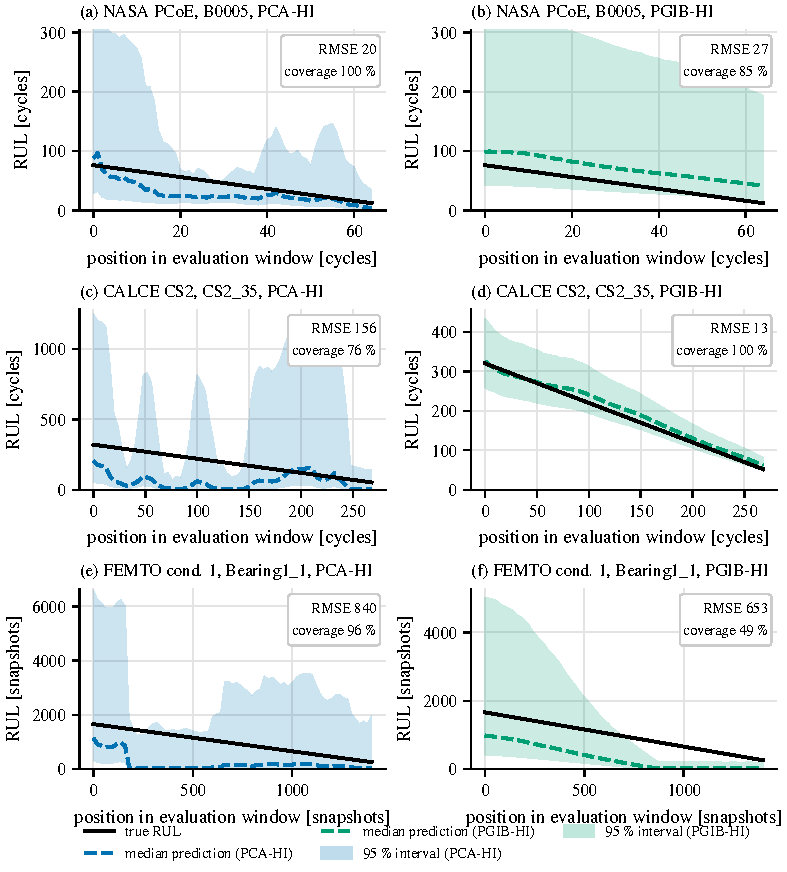
\includegraphics[width=\textwidth]{../figs/fig_bench}
\caption{Example RUL predictions with $95\%$ intervals on one held-out unit per data set (NASA B0005, CALCE CS2\_35, FEMTO Bearing1\_1), for PCA-HI (left) and PGIB (right); each panel gives the RMSE and the coverage on that unit.}
\label{fig:benchv1}
\end{figure}

\paragraph{Results under P1} The outcome depends on the data set (Tables~\ref{tab:benchv1} and \ref{tab:benchbv1}, Figure~\ref{fig:benchv1}), and the age-only baseline is needed to read it. On NASA the RMSE of the age-only baseline is $39.8$ cycles; PCA-HI ($17.8$), the Geo-opt HI ($21.9$), the $\beta$-VAE ($30.8$) and VIB ($33.3$) outperform it, whereas the PGIB ($47.6$) does not, and its intervals cover only $42\%$ of the true RULs. On CALCE the RMSE of the age-only baseline is $49.3$; only the PGIB ($33.0$) outperforms it clearly, while PCA-HI, the Geo-opt HI and the $\beta$-VAE ($117$ to $164$) are considerably worse than the age-only baseline. With the two $0.5$C-discharge cells added, the PGIB keeps the lowest RMSE ($50.4$) but its margin over the age-only baseline ($54.7$) is only $8\%$. On bearings the RMSE of the age-only baseline ($602$ and $664$ snapshots for conditions 1 and 2) is comparable to the standard deviation of the pooled RUL, and most HIs do no better: the PGIB has the lowest RMSE in condition 1 ($524.5$, $13\%$ below the age-only baseline) but gives almost no benefit in condition 2 ($621.8$ against $664$). Two long-lived units dominate the pooled error in condition 2.

The ablations (in the supplied result files) support the bottleneck on all five sets (for example RMSE $54.4\to47.6$ on NASA and $42.3\to33.0$ on CALCE) and the epistemic drift variance for coverage (for example $14\to42\%$ on NASA). The physics prior helps on CALCE and FEMTO condition 1 but not on NASA or FEMTO condition 2. With only three to six training units per fold, the validation signal that selects the encoder is itself noisy; on NASA it chose the strongest compression ($\beta=30$), at the edge of the grid, in all eight selections.

\paragraph{Geometric scores versus error} Across the five HIs of each data set, the rank correlation between the geometric score $\Mon+\mathrm{Tre}+\mathrm{Pro}$ and the RMSE is $+0.90$ on NASA (a higher geometric score goes with a larger error), $-1.00$ on CALCE, $-0.90$ on six-cell CALCE, $-0.60$ on FEMTO condition 1 and $+0.60$ on condition 2. The geometric criteria therefore did not rank the HIs consistently by prognostic error. This is an association over five methods per data set and not evidence for the mechanism of Theorem~\ref{thm:paradox}: the VIB and PGIB HIs have $\Mon\approx\mathrm{Tre}\approx1$ because their velocity is constrained to be positive, not because of a squeeze.



\section{Figures and tables moved out of the paper}
\label{sec:moved}
These figures and tables duplicate numbers that the paper gives in its text and in other tables.

\begin{figure}[!tb]
\centering
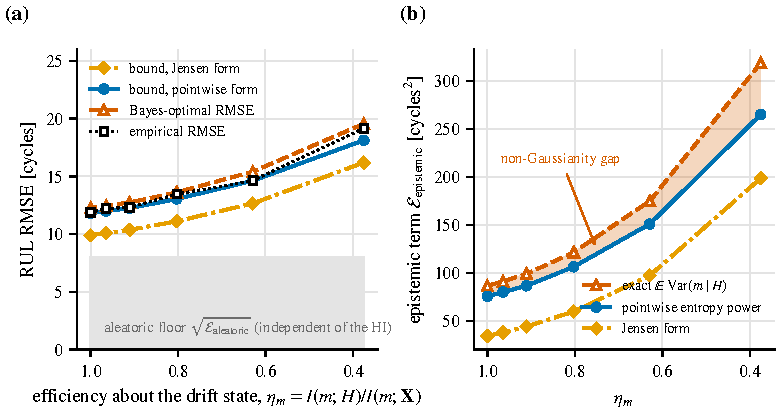
\includegraphics[width=\textwidth]{../figs/fig_bound}
\caption{Physics-constrained bound as the HI loses information (decreasing $\eta_m$). (a) RMSE of the bounds and estimators. (b) Epistemic term; the shaded area is the non-Gaussianity gap.}
\label{fig:bounds}
\end{figure}

\begin{figure}[!tb]
\centering
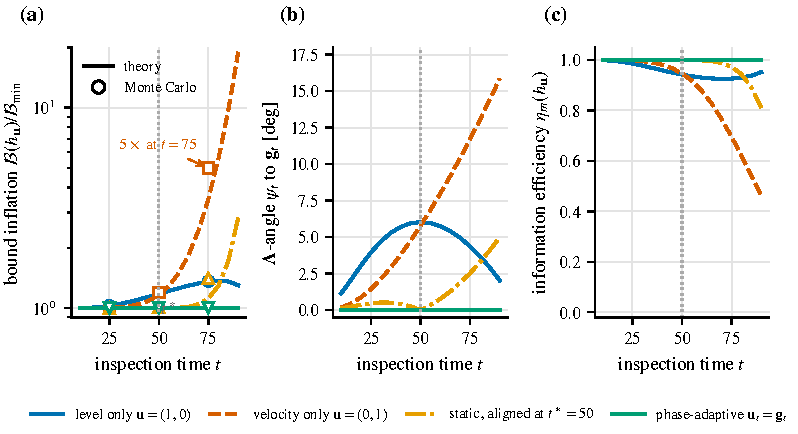
\includegraphics[width=\textwidth]{../figs/fig_angular}
\caption{Angular loss relation for scalar linear HIs. (a) Factor by which the bound increases. (b) Angle to the optimal direction $\mathbf g_t$ at the fixed operating point. (c) Information efficiency $\eta_m$. The static HI is aligned at $t^\ast=50$; the stage-adaptive HI uses the stage-wise gradient at the prior mean.}
\label{fig:angulars}
\end{figure}

\begin{figure}[!tb]
\centering
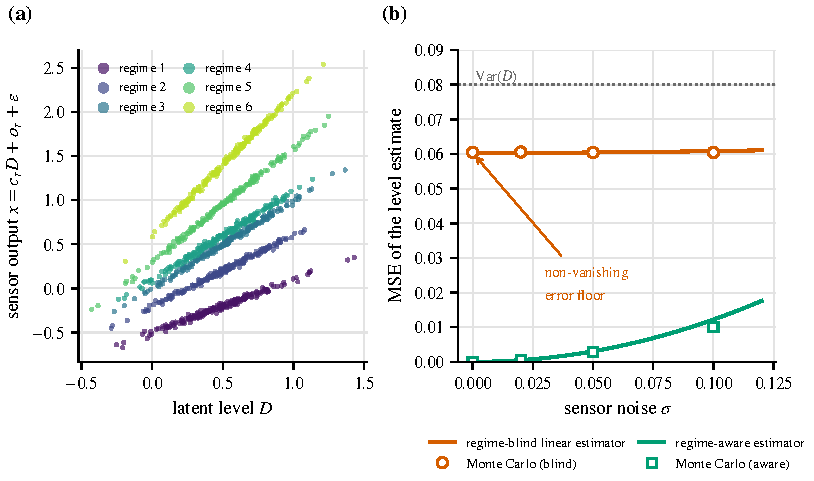
\includegraphics[width=\textwidth]{../figs/fig_regime}
\caption{Regime-blind estimation in the six-regime example. (a) Sensor output against latent level for each regime. (b) Error of the regime-blind and regime-aware estimators: formula (lines) and simulation (markers).}
\label{fig:regimes}
\end{figure}

\begin{table}[!htbp]
\caption{Template shrinkage of the ridge HI: monotonicity and information lower bound (nats).}
\centering\small
\adjustbox{max width=\linewidth}{\begin{tabular}{l l c c c c c c c}
\hline
Subset & & $\gamma=0.0$ & $\gamma=0.5$ & $\gamma=0.9$ & $\gamma=0.97$ & $\gamma=0.99$ & $\gamma=0.995$ & $\mathrm{Mon}_\infty$ (predicted) \\
\hline
FD001 & $\mathrm{Mon}$ & 0.24 & 0.34 & 0.54 & 0.56 & 0.55 & 0.55 & 0.55 \\
 & certificate & 0.31 & 0.28 & 0.21 & 0.09 & -0.06 & -0.08 & \\
FD002 & $\mathrm{Mon}$ & 0.19 & 0.28 & 0.54 & 0.58 & 0.58 & 0.58 & 0.61 \\
 & certificate & 0.21 & 0.20 & 0.18 & 0.11 & 0.00 & -0.06 & \\
FD003 & $\mathrm{Mon}$ & 0.16 & 0.22 & 0.40 & 0.41 & 0.42 & 0.42 & 0.41 \\
 & certificate & 0.10 & 0.10 & 0.10 & 0.07 & 0.02 & -0.07 & \\
FD004 & $\mathrm{Mon}$ & 0.13 & 0.18 & 0.36 & 0.41 & 0.41 & 0.41 & 0.41 \\
 & certificate & 0.17 & 0.18 & 0.16 & 0.13 & 0.07 & 0.00 & \\
\hline
\end{tabular}
}
\label{tab:rdsqueezes}
\end{table}

\begin{table}[!htbp]
\caption{Direction of a scalar linear HI: range of stage-optimal angles, best static angle, and worst-stage RMSE ratios to the direction chosen separately at each stage.}
\centering\small
\adjustbox{max width=\linewidth}{\begin{tabular}{l l c c c c c}
\hline
Subset & stages & optimal angle [deg] & static angle [deg] & static / free & level only / free & velocity only / free \\
\hline
FD001 & life fraction & 43--70 & 70 & 1.019 & 1.18 & 1.07 \\
FD001 & age & 33--69 & 60 & 1.021 & 1.20 & 1.18 \\
FD002 & life fraction & 18--66 & 55 & 1.002 & 1.13 & 1.05 \\
FD002 & age & 21--56 & 45 & 1.037 & 1.19 & 1.29 \\
FD003 & life fraction & 11--33 & 20 & 1.003 & 1.05 & 1.16 \\
FD003 & age & 6--35 & 25 & 1.025 & 1.08 & 1.38 \\
FD004 & life fraction & 1--20 & 5 & 1.007 & 1.02 & 1.10 \\
FD004 & age & 9--37 & 15 & 1.018 & 1.05 & 1.33 \\
\hline
\end{tabular}
}
\label{tab:rdstages}
\end{table}

\begin{figure}[!tb]
\centering
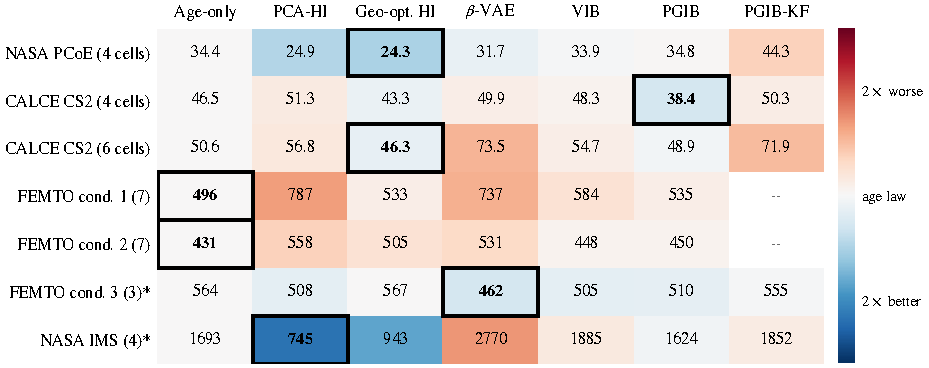
\includegraphics[width=\textwidth]{../figs/fig_small}
\caption{RMSE of the compared HIs on the seven small data sets (cycles for batteries, $10$~s snapshots for bearings). Colour: ratio to the age-only baseline; frame: lowest value of each row; cond.: operating condition; number of units in brackets; $^\ast$: sets not used in the design.}
\label{fig:smalls}
\end{figure}

\begin{table}[!htbp]
\caption{Cross-validated age-conditional information lower bounds (nats, $95\%$ bootstrap interval); $\bar h(T\mid t)$: mean conditional entropy. Sensors: raw sensors (engines) or charging features (cells); Capacity: reference predictor on the discharge capacity (cells).}
\centering\scriptsize
\adjustbox{max width=\linewidth}{\begin{tabular}{l c c c c c c c c c }
\hline
Subset & Units & $\bar h(T\mid t)$ & Age only (control) & Ridge HI & PCA-HI & Level only & Slope only & Sensors & Capacity (ref.) \\
\hline
FD001 & 100 & 5.11 & -0.11 [-0.28, 0.08] & 0.31 [0.20, 0.44] & 0.25 [0.13, 0.37] & 0.07 [-0.10, 0.24] & 0.17 [0.01, 0.32] & 0.22 [0.06, 0.38] & -- \\
FD002 & 260 & 5.11 & -0.11 [-0.22, -0.01] & 0.21 [0.13, 0.30] & 0.19 [0.11, 0.27] & 0.11 [0.03, 0.21] & 0.11 [0.01, 0.20] & 0.16 [0.08, 0.25] & -- \\
FD003 & 100 & 5.64 & -0.22 [-0.37, -0.03] & 0.10 [-0.05, 0.28] & 0.08 [-0.07, 0.25] & 0.06 [-0.09, 0.24] & 0.00 [-0.13, 0.16] & 0.20 [0.04, 0.40] & -- \\
FD004 & 249 & 5.52 & -0.12 [-0.24, -0.00] & 0.18 [0.06, 0.31] & 0.02 [-0.11, 0.14] & 0.14 [0.01, 0.28] & 0.02 [-0.10, 0.14] & 0.25 [0.13, 0.38] & -- \\
\hline
HUST & 77 & 7.11 & -0.02 [-0.14, 0.11] & 0.30 [0.19, 0.43] & 0.52 [0.42, 0.64] & 0.18 [0.06, 0.31] & 0.11 [0.01, 0.22] & 0.67 [0.57, 0.80] & 0.59 [0.48, 0.70] \\
MATR & 169 & 6.94 & -0.27 [-0.46, -0.05] & 0.32 [0.17, 0.51] & 0.34 [0.17, 0.54] & 0.24 [0.07, 0.44] & -0.03 [-0.21, 0.19] & 0.61 [0.42, 0.79] & 0.29 [0.09, 0.49] \\
\hline
\end{tabular}
}
\label{tab:rdcerts}
\end{table}

\begin{table}[!htbp]
\caption{RMSE of a linear estimator of the life fraction. Blind: without normalisation by regime (engines) or by the cell's own early cycles (cells).}
\centering\small
\begin{tabular}{l c c c c}
\hline
Subset & Regimes & Blind & Normalised & Regime-specific weights \\
\hline
FD001 & 1 & 0.139 & 0.139 & 0.139 \\
FD002 & 6 & 0.148 & 0.137 & 0.136 \\
FD003 & 1 & 0.156 & 0.156 & 0.156 \\
FD004 & 6 & 0.199 & 0.165 & 0.164 \\
HUST & one per cell & 0.136 & 0.115 & -- \\
MATR & one per cell & 0.179 & 0.142 & -- \\
\hline
\end{tabular}

\label{tab:rdregimes}
\end{table}

\begin{table}[!htbp]
\caption{Age-conditional information lower bounds (nats) of the benchmark methods on the official test engines. $^\dagger$: the age-only control fails.}
\centering\scriptsize
\adjustbox{max width=\linewidth}{\begin{tabular}{l c c c c }
\hline
Method & FD001 & FD002 & FD003$^\dagger$ & FD004 \\
\hline
$\bar h(T\mid t)$ & 5.09 & 5.07 & 5.61 & 5.47 \\
\hline
Age-only baseline (control) & 0.07 [-0.04, 0.20] & 0.01 [-0.07, 0.09] & 0.33 [0.23, 0.44] & 0.05 [-0.02, 0.13] \\
PCA-HI & 0.59 [0.49, 0.72] & 0.29 [0.21, 0.39] & 0.67 [0.54, 0.85] & 0.26 [0.19, 0.35] \\
Geo-opt HI & 0.58 [0.48, 0.71] & 0.23 [0.13, 0.36] & 1.10 [0.94, 1.30] & 0.66 [0.55, 0.76] \\
Ridge HI & 0.41 [0.26, 0.58] & 0.27 [0.17, 0.39] & 0.90 [0.77, 1.05] & 0.62 [0.54, 0.71] \\
$\beta$-VAE & 0.59 [0.47, 0.72] & 0.24 [0.16, 0.34] & 0.49 [0.35, 0.65] & 0.22 [0.14, 0.31] \\
VIB & 0.15 [0.01, 0.32] & 0.06 [-0.01, 0.14] & 0.57 [0.45, 0.74] & 0.11 [0.02, 0.22] \\
PGIB, integrating (10 seeds) & 0.14 [-0.02, 0.32] & 0.07 [-0.01, 0.16] & 0.49 [0.37, 0.63] & 0.19 [0.08, 0.30] \\
PGIB-KF (10 seeds) & 0.61 [0.45, 0.82] & 0.28 [0.18, 0.37] & 1.04 [0.87, 1.22] & 0.48 [0.39, 0.56] \\
PGIB-KFR (10 seeds) & 0.43 [0.28, 0.62] & 0.28 [0.20, 0.37] & 0.84 [0.73, 0.98] & 0.59 [0.51, 0.69] \\
\hline
\end{tabular}
}
\label{tab:rdtests}
\end{table}

\begin{table}
\caption{Estimation of $\etaPIE$ with the Kraskov--St\"ogbauer--Grassberger estimator ($k=5$, $100$ replications) in a Gaussian model with known mutual information; $n$ is the sample size.}
\centering\small
\begin{tabular}{r c c c c}
\hline
$n$ & $\hat I(T;\mathbf X)$ & $\hat I(T;H)$ & $\hat\eta_{\rm info}$ (mean $\pm$ standard deviation) & fraction $\hat\eta_{\rm info}>1$ \\
\hline
100 & 0.23 & 0.59 & $2.72\pm0.74$ & 1.00 \\
300 & 0.33 & 0.68 & $2.10\pm0.25$ & 1.00 \\
1000 & 0.43 & 0.71 & $1.65\pm0.09$ & 1.00 \\
3000 & 0.51 & 0.71 & $1.40\pm0.04$ & 1.00 \\
\hline
\multicolumn{5}{l}{true values: $I(T;\mathbf X)=1.00$, $I(T;H)=0.70$, $\eta_{\rm info}=0.70$ (nats)}\\
\end{tabular}

\label{tab:exp5s}
\end{table}

\begin{thebibliography}{42}
\bibitem{si2011} X.-S. Si, W. Wang, C.-H. Hu, D.-H. Zhou, Remaining useful life estimation -- a review on the statistical data driven approaches, Eur. J. Oper. Res. 213 (2011) 1--14. \url{https://doi.org/10.1016/j.ejor.2010.11.018}
\bibitem{lei2018} Y. Lei, N. Li, L. Guo, N. Li, T. Yan, J. Lin, Machinery health prognostics: a systematic review from data acquisition to RUL prediction, Mech. Syst. Signal Process. 104 (2018) 799--834. \url{https://doi.org/10.1016/j.ymssp.2017.11.016}
\bibitem{javed2017} K. Javed, R. Gouriveau, N. Zerhouni, State of the art and taxonomy of prognostics approaches, trends of prognostics applications and open issues towards maturity at different technology readiness levels, Mech. Syst. Signal Process. 94 (2017) 214--236. \url{https://doi.org/10.1016/j.ymssp.2017.01.050}
\bibitem{zio2022} E. Zio, Prognostics and health management (PHM): where are we and where do we (need to) go in theory and practice, Reliab. Eng. Syst. Saf. 218 (2022) 108119. \url{https://doi.org/10.1016/j.ress.2021.108119}
\bibitem{li2018} X. Li, Q. Ding, J.-Q. Sun, Remaining useful life estimation in prognostics using deep convolution neural networks, Reliab. Eng. Syst. Saf. 172 (2018) 1--11. \url{https://doi.org/10.1016/j.ress.2017.11.021}
\bibitem{whitmore1995} G.A. Whitmore, Estimating degradation by a Wiener diffusion process subject to measurement error, Lifetime Data Anal. 1 (1995) 307--319. \url{https://doi.org/10.1007/BF00985762}
\bibitem{lee2006} M.-L.T. Lee, G.A. Whitmore, Threshold regression for survival analysis: modeling event times by a stochastic process reaching a boundary, Stat. Sci. 21 (2006) 501--513. \url{https://doi.org/10.1214/088342306000000330}
\bibitem{aven2021} T. Aven, The reliability science: its foundation and link to risk science and other sciences, Reliab. Eng. Syst. Saf. 215 (2021) 107863. \url{https://doi.org/10.1016/j.ress.2021.107863}
\bibitem{coble2009} J. Coble, J.W. Hines, Identifying optimal prognostic parameters from data: a genetic algorithms approach, in: Annu. Conf. of the Prognostics and Health Management Society, vol. 1, 2009.
\bibitem{javed2013} K. Javed, R. Gouriveau, N. Zerhouni, P. Nectoux, A feature extraction procedure based on trigonometric functions and cumulative descriptors to enhance prognostics modeling, in: Proc. IEEE Conf. on Prognostics and Health Management, 2013, pp. 1--7. \url{https://doi.org/10.1109/ICPHM.2013.6621413}
\bibitem{zhang2016} B. Zhang, L. Zhang, J. Xu, Degradation feature selection for remaining useful life prediction of rolling element bearings, Qual. Reliab. Eng. Int. 32 (2016) 547--554. \url{https://doi.org/10.1002/qre.1771}
\bibitem{kingma2014} D.P. Kingma, M. Welling, Auto-encoding variational Bayes, in: Proc. Int. Conf. on Learning Representations, 2014. arXiv:1312.6114
\bibitem{severson2019} K.A. Severson, et al., Data-driven prediction of battery cycle life before capacity degradation, Nat. Energy 4 (2019) 383--391. \url{https://doi.org/10.1038/s41560-019-0356-8}
\bibitem{folks1978} J.L. Folks, R.S. Chhikara, The inverse Gaussian distribution and its statistical application -- a review, J. R. Stat. Soc. B 40 (1978) 263--275. \url{https://doi.org/10.1111/j.2517-6161.1978.tb01039.x}
\bibitem{chhikara1989} R.S. Chhikara, J.L. Folks, {\it The Inverse Gaussian Distribution: Theory, Methodology, and Applications}, Marcel Dekker, New York, 1989.
\bibitem{tweedie1957} M.C.K. Tweedie, Statistical properties of inverse Gaussian distributions. I, Ann. Math. Stat. 28 (1957) 362--377. \url{https://doi.org/10.1214/aoms/1177706964}
\bibitem{tang2014} S. Tang, C. Yu, X. Wang, X. Guo, X. Si, Remaining useful life prediction of lithium-ion batteries based on the Wiener process with measurement error, Energies 7 (2014) 520--547. \url{https://doi.org/10.3390/en7020520}
\bibitem{gebraeel2005} N.Z. Gebraeel, M.A. Lawley, R. Li, J.K. Ryan, Residual-life distributions from component degradation signals: a Bayesian approach, IIE Trans. 37 (2005) 543--557. \url{https://doi.org/10.1080/07408170590929018}
\bibitem{wang2010} X. Wang, Wiener processes with random effects for degradation data, J. Multivariate Anal. 101 (2010) 340--351. \url{https://doi.org/10.1016/j.jmva.2008.12.007}
\bibitem{sankararaman2013} S. Sankararaman, K. Goebel, Why is the remaining useful life prediction uncertain?, in: Annu. Conf. of the Prognostics and Health Management Society, vol. 5, 2013. \url{https://doi.org/10.36001/phmconf.2013.v5i1.2263}
\bibitem{lakshminarayanan2017} B. Lakshminarayanan, A. Pritzel, C. Blundell, Simple and scalable predictive uncertainty estimation using deep ensembles, in: Advances in Neural Information Processing Systems, vol. 30, 2017. arXiv:1612.01474
\bibitem{cover2006} T.M. Cover, J.A. Thomas, {\it Elements of Information Theory, 2nd ed.}, Wiley-Interscience, Hoboken, NJ, 2006.
\bibitem{tishby2000} N. Tishby, F.C. Pereira, W. Bialek, The information bottleneck method, arXiv:physics/0004057 (2000).
\bibitem{alemi2017} A.A. Alemi, I. Fischer, J.V. Dillon, K. Murphy, Deep variational information bottleneck, in: Proc. Int. Conf. on Learning Representations, 2017. arXiv:1612.00410
\bibitem{kraskov2004} A. Kraskov, H. St\"ogbauer, P. Grassberger, Estimating mutual information, Phys. Rev. E 69 (2004) 066138. \url{https://doi.org/10.1103/PhysRevE.69.066138}
\bibitem{paninski2003} L. Paninski, Estimation of entropy and mutual information, Neural Comput. 15 (2003) 1191--1253. \url{https://doi.org/10.1162/089976603321780272}
\bibitem{vantrees1968} H.L. Van Trees, {\it Detection, Estimation, and Modulation Theory, Part I}, Wiley, New York, 1968.
\bibitem{gill1995} R.D. Gill, B.Y. Levit, Applications of the van Trees inequality: a Bayesian Cram\'er--Rao bound, Bernoulli 1 (1995) 59--79. \url{https://doi.org/10.2307/3318681}
\bibitem{le2026jestch} H.H. Le, K.-A. Nguyen, Information-theoretic limits of health indicator construction for remaining useful life prediction, Eng. Sci. Technol. Int. J. 81 (2026) 102485. \url{https://doi.org/10.1016/j.jestch.2026.102485}
\bibitem{le2026mst} H.H. Le, K.-A. Nguyen, Generalization bounds and sample complexity for remaining useful life prediction from complete degradation trajectories, Meas. Sci. Technol. 37 (2026) 226203. \url{https://doi.org/10.1088/1361-6501/ae7109}
\bibitem{le2026ein} H.H. Le, K.-A. Nguyen, Charging phase health indicators for battery state-of-health estimation: a systematic comparison of CC, CV, and combined approaches under cross-battery validation, Eksploat. Niezawodn. -- Maint. Reliab. 28 (2026). \url{https://doi.org/10.17531/ein/220211}
\bibitem{bishop2006} C.M. Bishop, {\it Pattern Recognition and Machine Learning}, Springer, New York, 2006.
\bibitem{kalman1960} R.E. Kalman, A new approach to linear filtering and prediction problems, J. Basic Eng. 82 (1960) 35--45. \url{https://doi.org/10.1115/1.3662552}
\bibitem{durbin2012} J. Durbin, S.J. Koopman, {\it Time Series Analysis by State Space Methods, 2nd ed.}, Oxford University Press, Oxford, 2012.
\bibitem{vasicek1976} O. Vasicek, A test for normality based on sample entropy, J. R. Stat. Soc. B 38 (1976) 54--59. \url{https://doi.org/10.1111/j.2517-6161.1976.tb01566.x}
\bibitem{harvey1989} A.C. Harvey, {\it Forecasting, Structural Time Series Models and the Kalman Filter}, Cambridge University Press, Cambridge, 1989.
\bibitem{ma2022} G. Ma, et al., Real-time personalized health status prediction of lithium-ion batteries using deep transfer learning, Energy Environ. Sci. 15 (2022) 4083--4094. \url{https://doi.org/10.1039/D2EE01676A}
\bibitem{attia2020} P.M. Attia, et al., Closed-loop optimization of fast-charging protocols for batteries with machine learning, Nature 578 (2020) 397--402. \url{https://doi.org/10.1038/s41586-020-1994-5}
\bibitem{zhu2022} J. Zhu, et al., Data-driven capacity estimation of commercial lithium-ion batteries from voltage relaxation, Nat. Commun. 13 (2022) 2261. \url{https://doi.org/10.1038/s41467-022-29837-w}
\bibitem{tan2025} R. Tan, et al., BatteryLife: a comprehensive dataset and benchmark for battery life prediction, in: Proc. 31st ACM SIGKDD Conf. on Knowledge Discovery and Data Mining, vol. 2, 2025, pp. 5789--5800. \url{https://doi.org/10.1145/3711896.3737372}
\bibitem{bouthillier2021} X. Bouthillier, et al., Accounting for variance in machine learning benchmarks, Proc. Mach. Learn. Syst. 3 (2021) 747--769.
\bibitem{mauthe2024} F. Mauthe, C. Braun, J. Raible, P. Zeiler, M.F. Huber, Overview of publicly available degradation data sets for tasks within prognostics and health management, arXiv preprint (2024). arXiv:2403.13694
\end{thebibliography}

\end{document}
